% @HEADER
% ***********************************************************************
%            MatrixPortal: A Web-Based Computing Environment
%
% Under terms of Contract DE-AC04-94AL85000, there is a non-exclusive
% license for use of this work by or on behalf of the U.S. Government.
%
% This library is free software; you can redistribute it and/or modify
% it under the terms of the GNU Lesser General Public License as
% published by the Free Software Foundation; either version 2.1 of the
% License, or (at your option) any later version.
%
% This library is distributed in the hope that it will be useful, but
% WITHOUT ANY WARRANTY; without even the implied warranty of
% MERCHANTABILITY or FITNESS FOR A PARTICULAR PURPOSE.  See the GNU
% Lesser General Public License for more details.
%
% You should have received a copy of the GNU Lesser General Public
% License along with this library; if not, write to the Free Software
% Foundation, Inc., 59 Temple Place, Suite 330, Boston, MA 02111-1307
% USA
% ***********************************************************************
% @HEADER

\documentclass[11pt,relax]{SANDreport}
\usepackage{graphicx}
\usepackage{amsmath,amsfonts,amsthm}
\usepackage{amssymb}
\usepackage{enumerate}
\usepackage{rotating}


\usepackage{times}

\def\choicebox#1#2{\noindent$\hphantom{th}$\parbox[t]{1.8in}{\sf
#1}\parbox[t]{4.5in}{#2}\\[0.8em]}

\author{Sala, Phenow, Hu, Tuminaro}

\title{On the Development of Portals for Scientific Computing (DRAFT)}
\SANDnum{SAND2006-XXXX}
\SANDauthor{Sala, Phenow, Hu, Tuminaro}

\SANDprintDate{July 2006}
\SANDreleaseType{Unlimited Release}

\newcommand{\Trilinos}{Trilinos}
\newcommand{\TrilinosTM}{Trilinos \copyright}
\newcommand{\trilinos}{{\sc Trilinos}}
\newcommand{\ifpack}{{\sc Ifpack}}
\newcommand{\aztecoo}{{\sc AztecOO}}
\newcommand{\amesos}{{\sc Amesos}}
\newcommand{\epetra}{{\sc Epetra}}
\newcommand{\ml}{{\sc ML}}
\newcommand{\mb}[1]{{\mathbf {#1} }}
\newcommand{\teuchos}{{\sc Teuchos}}
\newcommand{\triutils}{{\sc Triutils}}
\newcommand{\metis}{{\sc METIS}}

\newcommand{\ie}{i.e., }
\newtheorem{assumption}{Assumption}[section]
\newtheorem{lemma}{Lemma}[section]
\newtheorem{proposition}{Proposition}[section]
\newtheorem{corollary}{Corollary}[section]
\newtheorem{theorem}{Theorem}[section]
\newtheorem{algorithm}{Algorithm}[section]
\newtheorem{definition}{Definition}[section]
\newtheorem{property}{Property}[section]

\newtheorem{remark}{Remark}
\newtheorem{problem}{Problem}

\def\choicebox#1#2{\noindent$\hphantom{th}$\parbox[t]{3.0in}{\sf
#1}\parbox[t]{3.35in}{#2}\\[0.8em]}

\begin{document}

\maketitle

\begin{abstract}
TO BE FIXED.... \\

Mathematical software is a subfield of computer science
characterized by a mixture of algorithms and numerics. Although elegant
theoretical results have been proved for a variety of problems, there is
typically no theory that can help to individuate the best algorithm for a
given problem or a set of problems. Often, proofs involve constants that
cannot, or is not convenient to be measured. Therefore, practical experience
is very often the last resort, and sometimes the only one for certain classes
of problems. Finding the best optimal algorithm in a given parameter space is
a tedious, error prone and long activity, which involves change of parameters,
and recording of results. As such, this activity can greatly benefit for
automation.  What we aim to present in this document is a set of tools that
can help to  evaluate the performances of scientific software, and in
particular of linear algebra libraries for high-performance computing. We
present the design and implementation of a  web interface that offers
a widely accessible, homogeneous
and easy-to-use graphical interface to a suite of linear algebra solvers.
This user-friendly interface promotes testing and
experimenting with a variety of state-of-the-art linear algebra libraries for
distributed sparse matrices.
\end{abstract}

\clearpage
\begin{center}
(page intentionally left blank)
\end{center}

\SANDmain

\tableofcontents

\clearpage
\newpage


% ------------------------------------------------------------------------- %
\section{Introduction}
% ------------------------------------------------------------------------- %

In the language of the World Wide Web (WWW), a {\sl portal}, or portal site,
is the site that users visit first. As its name stands for, it acts as a
doorway to all the resources of a given subject. Typically, a portal gives a
single, coherent view of information aggregated from disparate sources or
providers. 

Here, we are investigating the issues related to the development
and implementation of a portal for scientific computing. Therefore, we will
only consider {\sl vertical portal}, developed for a specified audience ---
that is, scientific computing. Although the ideas we present can in principle
be applied to a vast group of software projects, we will focus our attention
to sparse linear algebra.

With the term {\sl portal for scientific computing} we mean a web-based
interface to access high-performance software libraries. Among several
possible choices, we consider the Trilinos project~\cite{trilinos}
as concrete implementation
of our model. However, other projects (like PETSc~\cite{petsc-guide} 
                                       or Hypre~\cite{hypre}) could
straightforwardly be included in our portal.

MatrixPortal is intended to be a generic
toolkit that enables users to quickly test and get experience. The Web
interface encapsulates, in a high level of abstraction, the most prominent
features of the supported libraries. By offering a service like the
MatrixPortal, we hope to make our work
accessible to a larger target audience, and to receive feedback from the user
community.

We design our portal as a Web service. The Web Web standards have been
conceived to support interoperability, i.e., independence of the transport
protocols, programming languages, programming models, and system software.
Being based on industry standards like XML and HTML, a portal does not require
any special purpose hardware or software.  Since the services reside only on
the web server(s), the client software does not need to be updates every time
the web service is modified; changes to the interfaces simply need a "reload"
procedure.  The web service code never leaves the server, so property code is
protected. And, last but not least, Web services can be accessed from
everywhere and no special purpose interface is necessary.


\medskip

This report is organized as follows. Section~\ref{sec:design} presents the
design requirements and objectives of the portal. The computational model
is described in Section~\ref{sec:computational}.
Section~\ref{sec:navigation} outlines the navigation model.
Finally, Section~\ref{sec:concluding} reports the conclusions and the future
works.

% ------------------------------------------------------------------------- %
\section{Design Models for Scientific Computing Portals}
\label{sec:design}
% ------------------------------------------------------------------------- %

% ------------------------------------------------------------------------- %
\subsection{A Taxonomy for Scientific Computing Portals}
% ------------------------------------------------------------------------- %

{\bf To add references to other portals...}

We divide portals for scientific computing into two categories:
\begin{enumerate}
\setlength{\itemsep}{0pt}
\item {\sl Portals for the novice user,} which aim to minimize the investment
from this (casual) user, as well as the time required to move from the problem
specification to the data analysis. A possible usage of the novice mode is for
live presentations, or for teaching purposes.
\item {\sl Portal for the expert user,} where an extensive set of
functionalities is offered. In expert mode, the portal can be used as a
scientific computational tool, where real-life problems can be solved, and the
solution can be post-processed or sent to the user.
A key point to note in this category is the issue
of trust. Typically, expert users can upload their own problems, and possibly
define a custom script of compilation file. To avoid abuses or misuses of the
system, only certified users can receive the authorizations to access this
expert mode.
\end{enumerate}
Here, we describe the design and implementation issues for portal targeted to
novice users. The added value of these portals is the knowledge management
tools they offer.

{\bf Talk about grid-related portals}

\bigskip

MUST LOOK HERE: \verb!http://tyne.dl.ac.uk/GROWL/portal_guide/node3.html!

Talk about SANS (Self-Adapting Numerical Software)??? What else???

\verb!http://esc.dl.ac.uk/HPCPortal/!

Basic grid portal computing 
EPCC MHD portal, HPCGrid Portal 
Advance portal computing 
ASC Portal (Cactus Portal) 
Small scale grids (LSF, PBS, Condor) 
Toolkit approach (Globus, Legion, Unicore) 
Internet computing (Entropia, SETI@home)and peer-to-peer computing (Napster, Gnutella etc.)


www.gridforum.org

www.gridlab.org 

www.epcc.ed.ac.uk/ENACTS/

% ------------------------------------------------------------------------- %
\subsection{Why Scientific Computing Portals}
% ------------------------------------------------------------------------- %

Why should a novice portal be needed in the field of scientific computing? In
our opinion, the following motivations suggest that such a project could
benefit the research community:
\begin{itemize}
\setlength{\itemsep}{0pt}
\item Scientific libraries can require quite different amount
of knowledge to be unleashed. Software projects are sometimes large, and the
learning curve can be steep. Typically, it is not easy for the intended user
to load up his or her data and solve the corresponding problem with a new
library. This can slow down the testing, usage and acceptance of new 
projects. Being language-independent, and with no need to download or install
any software, a portal offers a demo version of the actual library which
requires a small amount of data, or no data at all if test problems are
selected.
%
\item For teaching and learning purposes, it can be of interest to move
smoothly from theoretical results to practical evidence.
Users interested only in the specific results 
(e.g., the iterations to converge for a given preconditioner) could benefit
from pop-down menus and common test problems.
some more parameters, thus encouraging experimentation. By using a portal,
the need to configure, compile and install is lifted. These steps are
generally challenging  for
the unexperienced user, and a time-consuming step for both unexperienced and
expert users. Besides, some configuration options may require additional
libraries.
%
\item Bug-tracking capabilities like Bugzilla~\cite{bugzilla} and
mailing lists help to create a sense of community, they are often not
effective enough to share data. A web portal can improve the communication
between users and developers: if a certain bug can be reproduced on the
portal, then developers will have all required data and access to the buggy
code. This can be a step forward {\sl collaborative computing}.
\item Comparing different versions, or compare the installed version with the
latest can become as easy as selecting one option in a list. Then, the user
can decide whether the new version deserves to be downloaded and installed or
not.
\end{itemize}

% ------------------------------------------------------------------------- %
\subsection{Portal Objectives}
% ------------------------------------------------------------------------- %

We are interesting in a user interface that favor the
experimentation process, and offer an extensive list of parameters to toggle
the behavior of the solvers, as well as a detailed help to guide users with
less experience. The approach is to offer a clear and uniform design, avoiding
everything that can be misinterpreted or can lead to confusion. The user
should be able to assign custom names to problem definitions, and perform 
a valid performance analysis. Performance analysis is required to help the 
decision-making processing for the user's application.  Conveying the
results in a clear and understandable way is a major objective of our work.

The design philosophy is that of a ``bag of services,'' that is, we aim to
offer a variety of solutions for a given problem. A user interested in using
the portal does not have to adopt any particular programming model or
language, to learn or read any documentation or to configure and install any
software.

% ------------------------------------------------------------------------- %
\subsection{Portal Requirements}
% ------------------------------------------------------------------------- %

The requirements for users are:
\begin{itemize}
\setlength{\itemsep}{0pt}
\item flexibility;
\item scalability;
\item low latency.
\end{itemize}
The requirements for managers are:
\begin{itemize}
\setlength{\itemsep}{0pt}
\item extensibility. Only a minimal investment should be required to add new
\item need to track and archive user information;
features.
\end{itemize}

% ------------------------------------------------------------------------- %
\section{The Portal from the User's Perspective}
\label{sec:navigation}
% ------------------------------------------------------------------------- %

The navigation of the web portal in the novice mode is reported in
Figure~\ref{fig:navigation}. These steps are:
\begin{itemize}
\setlength{\itemsep}{0pt}
\item {\sl selection of the problems of interest};
\item {\sl data checking};
\item {\sl selection of the solution parameters and evaluation criterion}.
In this step, the user selects the solution strategy, and specifies all the
parameters of interest. Also, an evaluation strategy is chosen. Since we are
targeting linear algebra applications, the evaluation parameter can be one of
the following: iterations, CPU time for construction and solution, or
estimated condition number (if available).
\item {\sl computation};
\item {\sl analysis of the results}.
\end{itemize}

\begin{figure}
\begin{center}
\begin{tabular}{c c c}
%
\begin{tabular}{| p{3.5cm} |}
\hline \\ Setup problems \\  \\ \hline
\end{tabular} 
& $\Rightarrow$ & 
%
\begin{tabular}{| p{3.5cm} |}
\hline \\ Analyze data\\ \\ \hline
\end{tabular}  \\
% - newline - %
               &               & $\Downarrow$ \\
% - newline - %
\begin{tabular}{| p{3.5cm} |}
\hline \\ Save results in XML\\ \\ \hline
\end{tabular}  
&  &
\begin{tabular}{| p{3.5cm} |}
\hline \\ Specify parameters\\ \\ \hline
\end{tabular}  \\
% - newline - %
$\Uparrow$     &               &    $\Downarrow$ \\
% - newline - %
\begin{tabular}{| p{3.5cm} |}
\hline \\ Analyze data\\ \\ \hline
\end{tabular}  & $\Leftarrow$ &
\begin{tabular}{| p{3.5cm} |}
\hline \\ Compute solutions\\ \\ \hline
\end{tabular}  \\
\end{tabular}
\end{center}
\caption{}
\label{fig:navigation}
\end{figure}

The portal is based on commodity Web technologies,
and it can be run by anyone who has access to a Web browser with support for
HTML 3.0, JavaScript 1.1, and the SSL protocol.  No special plugins are
required, nor a Java machine is used. This increases its portability.

We now analyze in more details these phases.

The types of applications
are so numerous that it is not possible to have a standard approach on
measure. Indeed, the first step in performance evaluation is to select the
right model and measure, the right measurement environments, and the right
techniques.

The easiest way to define data is by {\sl Data generation}. Linear systems can
be created on-the-fly from a collection of predefined problems.

By {\sl data acquisition} we mean the act of gathering data from multiple data
sources. To successfully acquire data, a system must support well-recognized
protocols. We adopt the Harwell/Boeing format or the
EpetraExt::XML format.

By {\sl data management} refers to functionalities for dealing with the various
information types once they have been made accessible by the data acquisition
component. Those include:
\begin{itemize}
\setlength{\itemsep}{0pt}
\item a persistent data repository;
\item index capabilities for data stored;
\item search facilities.
\end{itemize}

By {\sl data analysis} we mean all the techniques that can be used to gain
insight from the results. Data analysis is the key step towards decision
making. 

% ------------------------------------------------------------------------- %
\section{The Portal from the Server's Perspective}
\label{sec:computational}
% ------------------------------------------------------------------------- %

An overview of the structure is reported in Figure~\ref{fig:design}.
Our portal is organized in a three-layer structure. While the user's interface
resides on the client, the middle layer and the solver layer can be located in
the same machine, or as two separate services. In the first case, we have a
Client-Server service, in the latter a Client-Server-Solver. The solver layer
could be located on the Grid; in this case we call the structure
Client-Server-Grid.

\begin{figure}
\begin{center}
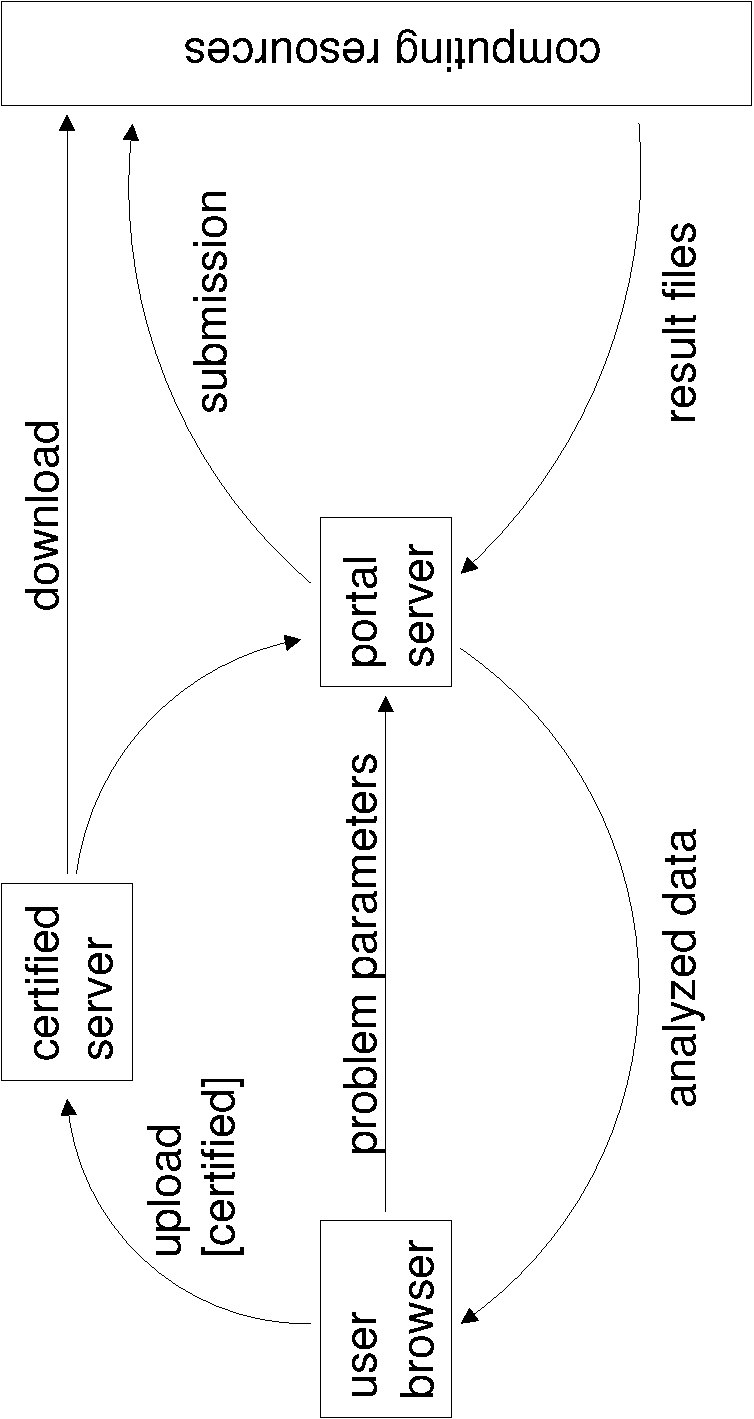
\includegraphics[width=14cm]{portal_design}
\caption{Design}
\end{center}
\label{fig:design}
\end{figure}

Ideally, the front-end would parse the proper specification from the source
code of the numerical software library and extract the required interface. To
make it simpler, we suppose that the library adhere to the following calling
sequence:
\begin{enumerate}
\setlength{\itemsep}{0pt}
\item parameters are declared
\item object is initialized
\item compute
\end{enumerate}
The information contained in the parameters are the parameter name, type, and
value. A check on admissible parameters is performed.

The list below describes the role of each tool composing the framework:
\begin{itemize}
\setlength{\itemsep}{0pt}
\item {\sl Data repository}. For authorized users, the portal might require
intensive exchange through the network. A data repository server acts as a
resource provider.
\item {\sl Solver-tier} (or back-end). The solver-tier consists of a python
scripts executing the tests.
\end{itemize}

\begin{figure}
\begin{center}
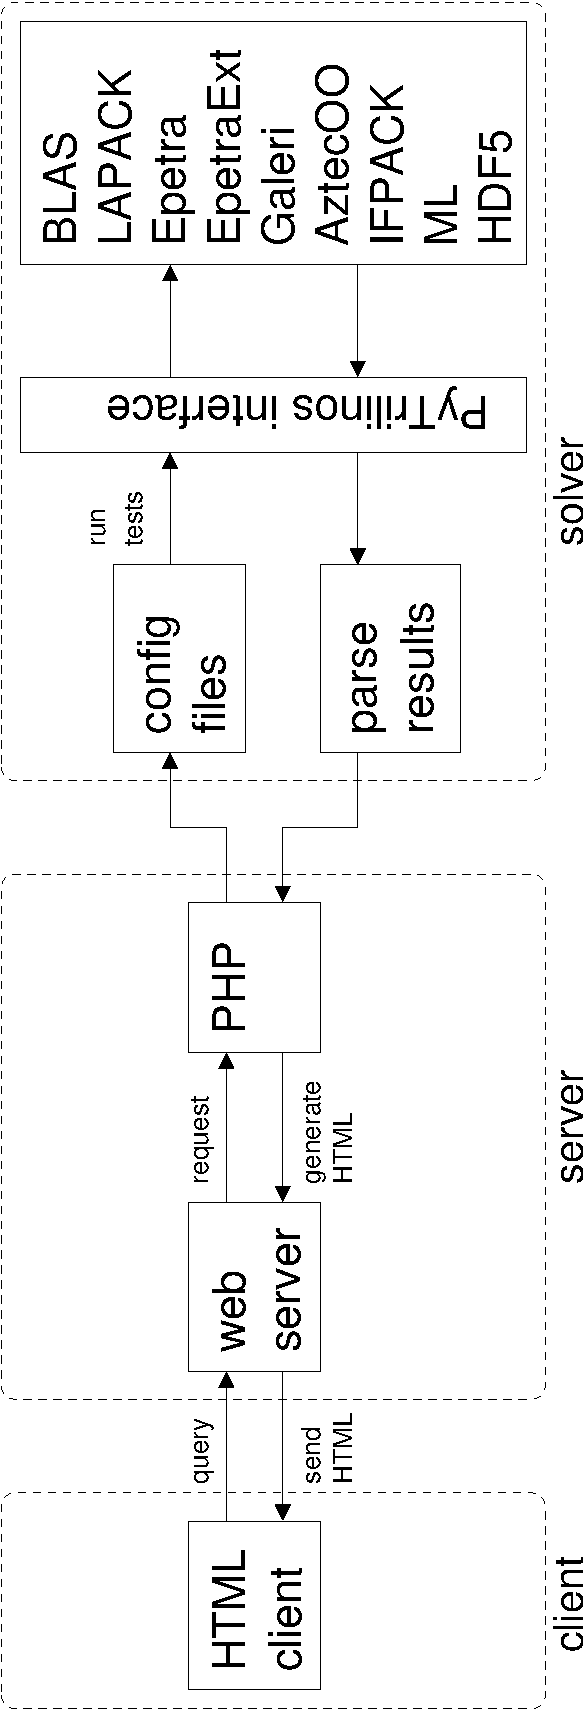
\includegraphics[width=14cm]{diagram}
\caption{Implementation diagram.}
\label{fig:design}
\end{center}
\end{figure}

Server's perspective:
\begin{itemize}
\item Web server (like Apache) with support for PHP version 4;
\item Python version 2.4 or more recent;
\item 
The middleware solution we use is based on Trilinos version 7.0 or more
recent. In particular, we use the Python interface to Trilinos, PyTrilinos.
PyTrilinos makes it possible to call several Trilinos packages, and therefore
BLAS, LAPACK, and several other libraries for distributed and serial linear
algebra.
\end{itemize}
The implementation diagram is reported in Figure~\ref{fig:design}.
  
% ------------------------------------------------------------------------- %
\section{Concluding Remarks}
\label{sec:concluding}
% ------------------------------------------------------------------------- %

We have described the design issues for a portal targeted to scientific
computing, with particular emphasis on sparse linear algebra. Motivations for
creating web portals are to ease experimentation, increase communication
between users and developers and within developers, scientific computation,
teaching, and diffision.

ease exploring new strategies with minimal investment. To allow the
casual user to explore the algorithms and ideas offered by a scientific
library and not by the implementation and installation details, it is
convenient to hide the complexity of the infrastructure and just offer a
fully-fledge, already configured web interface.

% ------------------------------------------------------------------------- %
\section*{Acknowledgments}
% ------------------------------------------------------------------------- %


% ------------------------------------------------------------------------- %
\bibliographystyle{plain}
\bibliography{biblio}
% ------------------------------------------------------------------------- %

\end{document}
